\documentclass{beamer}
\usetheme{tokitex}

\usepackage{graphics}
\usepackage{multirow}
\usepackage{tabto}

\usepackage[english,bahasa]{babel}
\newtranslation[to=bahasa]{Section}{Bagian}
\newtranslation[to=bahasa]{Subsection}{Subbagian}

\usepackage{listings, lstautogobble}
\usepackage{color}

\definecolor{dkgreen}{rgb}{0,0.6,0}
\definecolor{gray}{rgb}{0.5,0.5,0.5}
\definecolor{mauve}{rgb}{0.58,0,0.82}

\lstset{frame=tb,
  language=pascal,
  aboveskip=1mm,
  belowskip=1mm,
  showstringspaces=false,
  columns=fullflexible,
  keepspaces=true,
  basicstyle={\small\ttfamily},
  numbers=none,
  numberstyle=\tiny\color{gray},
  keywordstyle=\color{blue},
  commentstyle=\color{dkgreen},
  stringstyle=\color{mauve},
  breaklines=true,
  breakatwhitespace=true,
  autogobble=true
}

\title{Ekspresi dan \textit{Masukan/Keluaran}}
\author{Tim Olimpiade Komputer Indonesia}
\date{}

\begin{document}

\begin{frame}
\titlepage
\end{frame}

\begin{frame}
\frametitle{Pendahuluan}
Melalui dokumen ini, kalian akan:
\begin{itemize}
  \item Mengenal ekspresi.
  \item Mengenal masukan dan keluaran untuk program.
\end{itemize}
\end{frame}

\begin{frame}[fragile]
\frametitle{Kilas Balik: Assignment}
\begin{itemize}
  \item Membosankan sekali jika kita hanya bisa mengisi variabel dengan nilai yang pasti. 
  \item Kadang-kadang dibutuhkan hal yang lebih ekspresif. Contoh:
  \begin{lstlisting}
    a := 5;
    b := 2;
    jumlah := a + b;
  \end{lstlisting}
  \item Kenyataannya, hal ini dapat diwujudkan pada pemrograman!
  \item Perintah "a + b" biasa disebut sebagai \alert{ekspresi}.
\end{itemize}
\end{frame}

\section{Ekspresi}
\frame{\sectionpage}

\begin{frame}
\frametitle{Mengenal Ekspresi}
\begin{figure}
  \centering
  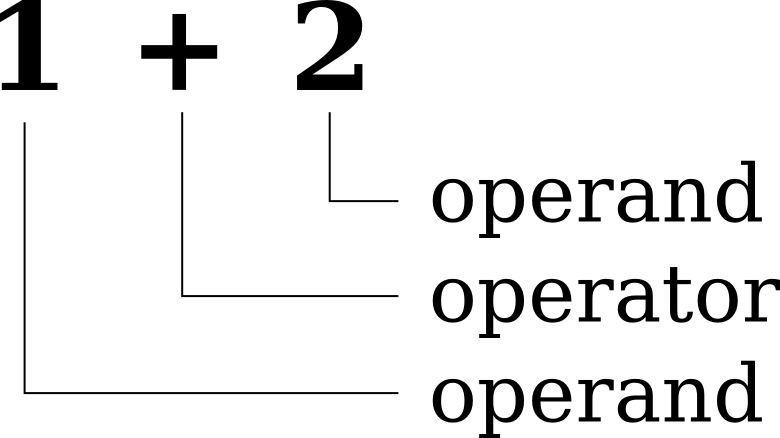
\includegraphics[width=4 cm]{asset/ekspresi.png}
\end{figure}
\begin{itemize}
  \item Ekspresi terdiri dari dua komponen: \alert{operator} dan \alert{operand}.
  \item Operand menyatakan nilai yang akan dioperasikan, misalnya bilangan atau suatu ekspresi lagi.
  \item Operator menyatakan bagaimana operand akan dioperasikan, apakah ditambah, dikali, atau dibagi?
\end{itemize}
\end{frame}

\begin{frame}
\frametitle{Mengenal Ekspresi (lanj.)}
Bisa juga dibentuk ekspresi bersarang, yaitu ekspresi yang operand-nya merupakan ekspresi lagi:
\begin{figure}
  \centering
  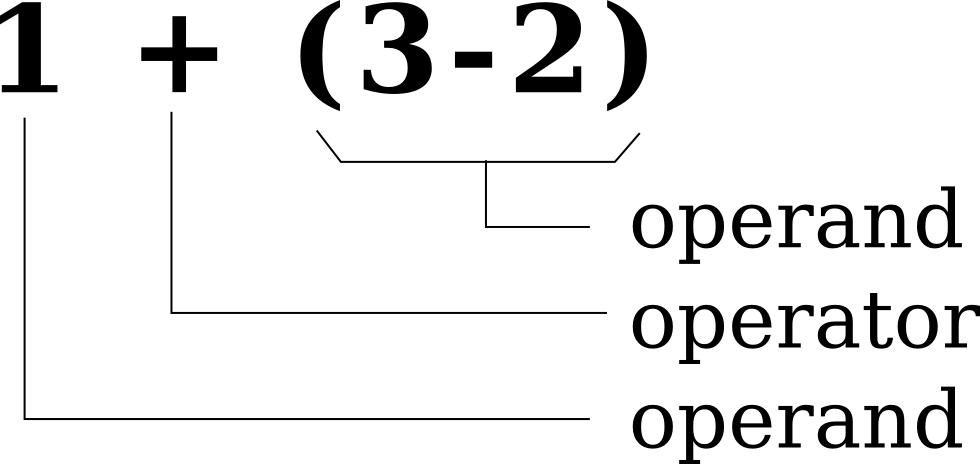
\includegraphics[width=5 cm]{asset/ekspresi-nested.png}
\end{figure}
\end{frame}

\begin{frame}
\frametitle{Operasi Numerik}
\begin{itemize}
  \item Operasi pada bilangan yang dapat dilakukan adalah penjumlahan (+), pengurangan (-), perkalian (*), pembagian (/), pembagian \textit{integer} (div), dan modulo (mod).
  \item Jika kedua operand merupakan bilangan bulat, hasil pengoperasian selalu bilangan bulat juga, kecuali untuk operasi pembagian yang selalu menghasilkan \textit{floating point}. Contoh:
  \begin{itemize}
    \item 3 - 1 = 2
    \item 10 / 5 = 2.0000000
    \item 7 / 2 = 3.5000000
  \end{itemize}
  \item Ketika setidaknya salah satu dari operand ada yang bertipe data \textit{floating point}, pengoperasian akan selalu menghasilkan \textit{floating point}.
\end{itemize}
\end{frame}

\begin{frame}
\frametitle{Operasi Numerik (lanj.)}
\begin{itemize}
  \item Operasi pembagian \textit{integer} didefinisikan sebagai: membagi, lalu dibulatkan ke bawah. Contoh:
  \begin{itemize}
    \item 7 div 2 = 3
    \item 10 div 2 = 5
    \item 3 div 5 = 0
  \end{itemize}
  \item Operasi modulo adalah mengambil sisa bagi dari operand pertama terhadap operand kedua. Contoh:
  \begin{itemize}
    \item 7 mod 2 = 1
    \item 10 mod 2 = 0
    \item 3 mod 5 = 3
    \item 8 mod 3 = 2
  \end{itemize}
  \item Operasi div dan mod hanya bisa dilakukan apabila kedua operand memiliki tipe data \alert{bilangan bulat}.
\end{itemize}
\end{frame}

\begin{frame}[fragile]
\frametitle{Contoh Program: kuadrat.pas}
\begin{itemize}
  \item Setelah memahami tentang operasi numerik, coba perhatikan program berikut dan cari tahu apa keluarannya!
  \begin{lstlisting}
    var
      a, b, c, x, hasil: longint;
    begin
      a := 1;
      b := 3;
      c := -2;
      x := 2;

      hasil := a*x*x + b*x + c;
      writeln('ax^2 + bx + c = ', hasil);
    end.
  \end{lstlisting}
\end{itemize}
\end{frame}

\begin{frame}
\frametitle{Prioritas Pengerjaan}
\begin{itemize}
  \item Seperti pada ilmu matematika, ada juga prioritas pengerjaan pada ekspresi numerik. Tabel berikut menunjukkan prioritasnya:

  \begin{tabular}{|c|c|}
  \hline Prioritas & Operasi \\
  \hline 1 & *,/,div,mod \\
  \hline 2 & +,- \\
  \hline
  \end{tabular}
  \item Jika ada beberapa operasi bersebelahan yang memiliki prioritas sama, operasi yang terletak di posisi lebih kiri akan dikerjakan lebih dahulu.
\end{itemize}
\end{frame}

\begin{frame}[fragile]
\frametitle{Contoh Program: numerik.pas}
\begin{itemize}
  \item Kita juga bisa menggunakan tanda kurung untuk mengatur prioritas pengerjaan suatu ekspresi.
  \item Perhatikan contoh berikut dan coba jalankan programnya:
  \begin{lstlisting}
    var
      hasil1, hasil2: longint;
    begin
      hasil1 := 3+5 div 4;
      hasil2 := (3+5) div 4;
      writeln(hasil1);
      writeln(hasil2);
    end.
  \end{lstlisting}
  \item Isi dari variabel hasil1 adalah 4, karena operasi "5 div 4" memiliki prioritas yang lebih tinggi untuk dikerjakan, dan menghasilkan nilai 1. Barulah "3 + 1" dilaksanakan kemudian.
\end{itemize}
\end{frame}

\begin{frame}
\frametitle{Fungsi Dasar Numerik}
Berikut fungsi dasar yang disediakan Pascal untuk membantu perhitungan:
\begin{itemize}
  \item \textbf{trunc}: mengambil bagian depan penanda desimal dari suatu bilangan pecahan. Contoh: \textbf{trunc(3.14)} akan menghasilkan 3 (sebuah \textit{integer}).
  \item \textbf{frac}: mengambil bagian belakang penanda desimal dari suatu bilangan pecahan. Contoh: \textbf{frac(3.14)} akan menghasilkan 0.14.
\end{itemize}
\end{frame}

\begin{frame}
\frametitle{Fungsi Dasar Numerik (lanj.)}
\begin{itemize}
  \item \textbf{round}: membulatkan suatu bilangan pecahan bilangan bulat terdekat (hasilnya adalah bilangan bertipe \textit{integer}). Contoh: \textbf{round(1.2)} akan menghasilkan 1, sementara \textbf{round(1.87)} akan menghasilkan 2.
  \item \textbf{sqr}: mengkuadratkan suatu bilangan. Contoh: \textbf{sqr(3)} akan menghasilkan 9.
  \item \textbf{sqrt}: mendapatkan akar kuadrat dari suatu bilangan. Contoh: \textbf{sqrt(9)} akan menghasilkan 3.00, dan \textbf{sqrt(3)} akan menghasilkan 1.73205....
\end{itemize}
\end{frame}

\begin{frame}
\frametitle{Fungsi Dasar Numerik (lanj.)}
\begin{block}{Catatan khusus untuk fungsi \textbf{round}}
Jika angka yang diberikan memiliki pecahan tepat setengah, pembulatan ditentukan dari angka sebelum penanda desimal. Jika ganjil, dilakukan pembulatan ke atas. Jika genap, dilakukan pembulatan ke bawah.

Contoh:
\begin{itemize}
\item \textbf{round(1.5)} = 2
\item \textbf{round(2.5)} = 2
\item \textbf{round(3.5)} = 4
\end{itemize}
\end{block}
\end{frame}

\begin{frame}[fragile]
\frametitle{Contoh Program: kuadrat2.pas}
\begin{itemize}
  \item Program kuadrat1.pas bisa ditulis juga dengan menggunakan fungsi \textbf{sqr}, sehingga menjadi:
  \begin{lstlisting}
    var
      a, b, c, x, hasil: longint;
    begin
      a := 1;
      b := 3;
      c := -2;
      x := 2;

      hasil := a*sqr(x) + b*x + c;
      writeln('ax^2 + bx + c = ', hasil);
    end.
  \end{lstlisting}
\end{itemize}
\end{frame}

\begin{frame}
\frametitle{Operasi Relasional}
\begin{itemize}
  \item Kita juga bisa melakukan operasi relasional, yaitu:
  \begin{itemize}
    \item kurang dari ($<$)
    \item lebih dari ($>$)
    \item sama dengan ($=$)
    \item kurang dari atau sama dengan ($<=$)
    \item lebih dari atau sama dengan ($>=$)
    \item tidak sama dengan ($<>$)
  \end{itemize}
  \item Operasi relasional harus melibatkan dua operand (ingat bahwa operand bisa jadi berupa ekspresi lagi), dan menghasilkan sebuah nilai kebenaran.
  \item Pada Pascal, nilai kebenaran dinyatakan dengan tipe data \alert{\textbf{boolean}}.
\end{itemize}
\end{frame}

\begin{frame}[fragile]
\frametitle{Contoh Program: relasional.pas}
\begin{itemize}
  \item Perhatikan contoh berikut dan coba jalankan programnya:
  \begin{lstlisting}
    begin
      writeln(2 > 1);
      writeln(2 < 1);
      writeln(2 = 1);
      writeln(2 >= 1);
      writeln(1 = 1);
      writeln(1 <> 1);
      writeln(1 <> 2);
    end.
  \end{lstlisting}
\end{itemize}
\end{frame}

\begin{frame}[fragile]
\frametitle{Operasi Relasional pada Floating Point}
\begin{itemize}
  \item Karena komputer tidak dapat secara sempurna menyimpan nilai \textit{floating point}, Anda perlu hati-hati saat membandingkan dua bilangan riil.
  \item Ekspresi berikut mungkin saja bernilai \textbf{FALSE}:
  \begin{lstlisting}
  (0.1 + 0.2) = 0.3
  \end{lstlisting}
  \item Sebab 0.1 + 0.2 bisa saja bernilai \textbf{0.30000000000000001}
\end{itemize}
\end{frame}

\begin{frame}
\frametitle{Operasi Relasional pada Floating Point (lanj.)}
\begin{itemize}
  \item Untuk memeriksa kesamaan antara dua nilai \textit{floating point}, biasanya dilibatkan suatu nilai toleransi.
  \item Misalnya, kedua nilai dianggap sama apabila selisih mereka kurang dari $10^{-8}$.
\end{itemize}
\end{frame}

\begin{frame}
\frametitle{Operasi Relasional (lanj.)}
\begin{itemize}
  \item Operasi relasional dapat dilakukan pada setiap tipe data ordinal, sehingga bisa juga diterapkan pada \textbf{char}.
  \item Perbandingan karakter dilakukan dengan membandingkan kode ASCII mereka, sehingga menjadi seperti membandingkan angka biasa.
  \item Contoh:
  \begin{itemize}
    \item 'a' $<$ 'b' akan bernilai \textbf{TRUE}
    \item 'a' $>$ 'z' bernilai \textbf{FALSE}
    \item 'A' $<$ 'a' akan bernilai \textbf{TRUE}
  \end{itemize}
\end{itemize}
\end{frame}

\begin{frame}
\frametitle{Operasi Relasional (string)}
\begin{itemize}
  \item Lebih jauh lagi, \textbf{string} sebenarnya merupakan untaian \textbf{char}. Operasi relasional juga bisa diterapkan pada \textbf{string} (meskipun \textbf{string} bukan tipe data ordinal).
  \item Pascal akan membandingkan karakter demi karakter dari kiri ke kanan. Begitu ditemukan ada perbedaan karakter, lebih kecil atau tidaknya suatu string ditentukan oleh karakter tersebut.
  \begin{itemize}
    \item Contohnya, 'aa' $<$ 'ab' akan bernilai \textbf{TRUE}.
  \end{itemize}
  \item Jika sampai salah satu string habis dan tidak ditemukan ada perbedaan karakter, maka stirng yang lebih pendek dianggap lebih kecil.
  \begin{itemize}
    \item Contohnya 'a' $<$ 'aa' bernilai \textbf{TRUE}.
  \end{itemize}
\end{itemize}
\end{frame}

\begin{frame}[fragile]
\frametitle{Contoh Program: relasional2.pas}
\begin{itemize}
  \item Perhatikan contoh berikut dan coba jalankan programnya:
    \begin{lstlisting}
      begin
        writeln('a' > 'A');
        writeln('a' < 'A');
        writeln('a' >= 'A');
        writeln('a' = 'A');

        writeln('a' < 'aa');
        writeln('abcb' > 'abca');
        writeln('abc' = 'abc');
        writeln('abc' <= 'abc');
      end.
    \end{lstlisting}
\end{itemize}
\end{frame}

\begin{frame}
\frametitle{Operasi Boolean}
\begin{itemize}
  \item Operasi \textbf{boolean} merupakan operasi yang hanya melibatkan nilai-nilai kebenaran. Terdiri atas: \textbf{not}, \textbf{and}, \textbf{or}, \textbf{xor}.
  \item Operasi-operasi ini sesuai dengan sebuah cabang ilmu matematika yang bernama "aljabar boolean".
  \item Operasi \alert{not} merupakan operasi \textit{unary}, artinya hanya melibatkan satu operand. Gunanya untuk membalik nilai kebenaran.
  \item Tabel berikut menunjukkan efek dari penggunaan \textbf{not}.
  \begin{tabular}{|c|c|}
  \hline a & not a \\
  \hline TRUE & FALSE \\
  \hline FALSE & TRUE \\
  \hline
  \end{tabular}
\end{itemize}
\end{frame}

\begin{frame}
\frametitle{Operasi Boolean (lanj.)}
\begin{itemize}
  \item Operasi \textbf{boolean} yang lainnya merupakan operasi \textit{binary}, yang artinya melibatkan dua operand.
  \item Tabel berikut menunjukkan efek dari penggunaan operator-operator tersebut:
  \begin{tabular}{|c|c|c|c|c|}
  \hline a & b & a and b & a or b & a xor b \\
  \hline TRUE & TRUE & TRUE & TRUE & FALSE \\
  \hline TRUE & FALSE & FALSE & TRUE & TRUE \\
  \hline FALSE & TRUE & FALSE & TRUE & TRUE\\
  \hline FALSE & FALSE & FALSE & FALSE & FALSE \\
  \hline
  \end{tabular}
\end{itemize}
\end{frame}

\begin{frame}
\frametitle{Operasi Boolean (lanj.)}
\begin{itemize}
  \item Prioritas pengerjaan dari operator \textbf{boolean} secara berurutan adalah: \textbf{not}, \textbf{and}, \textbf{or}, \textbf{xor}.
  \item Tanda kurung juga bisa digunakan untuk menentukan operasi mana yang perlu dijalankan terlebih dahulu. Bahkan sangat disarankan untuk selalu menggunakan tanda kurung untuk kejelasan.
\end{itemize}
\end{frame}

\begin{frame}[fragile]
\frametitle{Contoh Program: relasional3.pas}
\begin{itemize}
  \item Perhatikan contoh berikut dan coba jalankan programnya:
  \begin{lstlisting}
    begin
      writeln(2 > 1);
      writeln(not (2 > 1));
      writeln((2 > 1) and (3 > 1));
      writeln(((2 > 1) or (3 < 1)) and (1 = 1));
      writeln((1 <> 1) xor not (1 <> 1));
    end.
  \end{lstlisting}
  \item Perhatikan bahwa tanda kurung diperlukan dalam ekspresi "not (2 $>$ 1)". Dengan tanda kurung, "2 $>$ 1" akan dievaluasi terlebih dahulu, menghasilkan nilai \textbf{boolean}. Barulah operator \textbf{not} bisa mengolah nilai \textbf{boolean} tersebut.
\end{itemize}
\end{frame}

\section{Masukan dan Keluaran}
\frame{\sectionpage}

\begin{frame}[fragile]
\frametitle{Kilas Balik: kuadrat2.pas}
\begin{itemize}
  \item Sekarang coba lihat kembali program kuadrat2.pas:
  \begin{lstlisting}
    var
      a, b, c, x, hasil: longint;
    begin
      a := 1;
      b := 3;
      c := -2;
      x := 2;

      hasil := a*sqr(x) + b*x + c;
      writeln('ax^2 + bx + c = ', hasil);
    end.
  \end{lstlisting}
  \item Jika kita ingin mengganti nilai \textbf{x}, kode harus diganti, dikompilasi ulang, baru dijalankan kembali.
  \item Untuk menghasilkan keluaran yang bervariasi, perlu ada \newline masukan dari luar program.
\end{itemize}
\end{frame}

\begin{frame}
\frametitle{Membaca Masukan}
\begin{itemize}
  \item Diperlukan mekanisme untuk melakukan pembacaan masukan dari luar program.
  \item Masukan bagi suatu program bisa berasal dari berbagai sumber, misalnya \textit{standard input} atau \textit{file}.
  \item Pada Pascal, dikenal dua fungsi yang umum untuk membaca masukan: \alert{\textbf{read}} dan \alert{\textbf{readln}}.
\end{itemize}
\end{frame}

\begin{frame}[fragile]
\frametitle{Membaca Masukan: readln}
\begin{itemize}
  \item Lakukan modifikasi pada bagian \textbf{x := 2} menjadi \textbf{readln(x)}:
  \begin{lstlisting}
    var
      a, b, c, x, hasil: longint;
    begin
      a := 1;
      b := 3;
      c := -2;
      readln(x);

      hasil := a*sqr(x) + b*x + c;
      writeln('ax^2 + bx + c = ', hasil);
    end.
  \end{lstlisting}
  \item Kompilasi, dan jalankan program. Kemudian ketikkan angka 2, dan tekan enter.
  \item Selamat! Kalian berhasil membaca masukan!
\end{itemize}
\end{frame}

\begin{frame}[fragile]
\frametitle{Fungsi readln}
  \begin{itemize}
    \item Fungsi \textbf{readln} berguna untuk membaca masukan, dan nilainya dapat di-\textit{assign} ke dalam variabel.
    \item Cara kerja readln: pada berkas masukan, cari \textit{token} yang dapat dibaca berikutnya, lalu baca ambil nilainya.
    \item Yang dimaksud \textit{token} adalah serangkaian karakter non-spasi, misalnya huruf atau angka.
    \item Pada contoh sebelumnya, \textit{token} yang dimaksud adalah bilangan yang akan menjadi nilai variabel \textbf{x}.
  \end{itemize}
\end{frame}


\begin{frame}[fragile]
\frametitle{Membaca Masukan: read}
\begin{itemize}
  \item Sekarang ganti \textbf{readln(x)} menjadi \textbf{read(x)}:
  \begin{lstlisting}
    var
      a, b, c, x, hasil: longint;
    begin
      a := 1;
      b := 3;
      c := -2;
      read(x);

      hasil := a*sqr(x) + b*x + c;
      writeln('ax^2 + bx + c = ', hasil);
    end.
  \end{lstlisting}
  \item Kompilasi, dan jalankan program. Kemudian ketikkan angka 2, dan tekan enter.
  \item Hasilnya tetap sama. Lalu apa yang membedakan \textbf{readln} \\ dengan \textbf{read}?
\end{itemize}
\end{frame}

\begin{frame}[fragile]
\frametitle{Perbedaan readln dengan read}
Setelah \textbf{read} atau \textbf{readln} mencari \textit{token} berikutnya dan membacanya, yang terjadi selanjutnya adalah:
\begin{block}{readln}
  Program disiapkan untuk membaca masukan
   
  selanjutnya di \alert{baris berikutnya}.
\end{block}
\begin{block}{read}
  Program \alert{tidak} disiapkan untuk membaca masukan 
  
  selanjutnya di \alert{baris berikutnya}.
\end{block}
\end{frame}

\begin{frame}[fragile]
\frametitle{Perbedaan readln dengan read (lanj.)}
\begin{itemize}
  \item Artinya, jika kita ingin membaca masukan dengan format:
  \begin{itemize}
    \item Baris pertama berisi tiga bilangan bulat dipisahkan dengan sebuah spasi, yaitu a, b, dan c.
    \item Baris kedua berisi sebuah bilangan bulat, yaitu x.
  \end{itemize}
  \item Dapat digunakan:
  \begin{lstlisting}
    read(a);
    read(b);
    readln(c);
    readln(x);
  \end{lstlisting}
\end{itemize}
\end{frame}

\begin{frame}[fragile]
\frametitle{Perbedaan readln dengan read (lanj.)}
\begin{itemize}
  \item Boleh juga:
  \begin{lstlisting}
    read(a);
    read(b);
    read(c);
    read(x);
  \end{lstlisting}
  \item Ingat bahwa baik \textbf{read} maupun \textbf{readln} akan mencari \textit{token} berikutnya untuk dibaca, tanpa peduli di baris mana \textit{token} itu berada.
\end{itemize}
\end{frame}

\begin{frame}[fragile]
\frametitle{Perbedaan readln dengan read (lanj.)}
\begin{itemize}
  \item Namun hal ini tidak bisa dilakukan:
  \begin{lstlisting}
    readln(a);
    readln(b);
    readln(c);
    readln(x);
  \end{lstlisting}
  \item Sebab pada \textbf{readln}, setelah membaca \textit{token} pada suatu baris, sisa \textit{token} yang ada pada baris yang sama diabaikan dan langsung berpindah ke baris berikutnya.
  \item Akibatnya, \textit{token} yang seharusnya menjadi masukan bagi variabel \textbf{b} dan \textbf{c} terabaikan.
\end{itemize}
\end{frame}

\begin{frame}[fragile]
\frametitle{Perbedaan readln dengan read (lanj.)}
\begin{itemize}
  \item Sebagai alternatif, \textbf{readln} dan \textbf{read} juga bisa digunakan untuk membaca beberapa masukan pada suatu baris secara bersamaan.
  \item Contoh penggunaan yang benar:
  \begin{lstlisting}
    readln(a,b,c);
    readln(x);
  \end{lstlisting}
  atau
  \begin{lstlisting}
    read(a,b);
    readln(c);
    readln(x);
  \end{lstlisting}
\end{itemize}
\end{frame}

\begin{frame}[fragile]
\frametitle{Kegunaan Lain readln}
\begin{itemize}
  \item Fungsi \textbf{readln} dapat digunakan untuk memaksa program untuk berpindah baris dalam membaca masukan. 
  \item Caranya dengan mengosongkan variabel di dalam pemanggilan fungsi \textbf{readln}.
  \item Pada contoh yang sebelumnya, boleh juga digunakan cara membaca seperti ini:
  \begin{lstlisting}
    read(a,b,c);
    readln;
    readln(x);
  \end{lstlisting}
\end{itemize}
\end{frame}

\begin{frame}[fragile]
\frametitle{Membaca string}
\begin{itemize}
  \item Khusus untuk membaca \textit{string}, baik \textbf{read} maupun \textbf{readln} akan membaca satu baris penuh.
  \item Perhatikan program berikut:
  \begin{lstlisting}
    var
      s: string;
    begin
      readln(s);
      writeln('s = ', s);
    end.
  \end{lstlisting}
\end{itemize}
\end{frame}

\begin{frame}[fragile]
\frametitle{Membaca string (lanj.)}
\begin{itemize}
  \item Jika program tersebut diberi masukan:
  \begin{lstlisting}
    bebek 123
  \end{lstlisting}
  \item maka keluaran dari program tersebut adalah:
  \begin{lstlisting}
    s = bebek 123
  \end{lstlisting}
  \item Dari contoh ini, diketahui bahwa variabel \textbf{s} berisi "bebek 123".
\end{itemize}
\end{frame}

\begin{frame}[fragile]
\frametitle{Membaca string (lanj.)}
\begin{itemize}
  \item Bagaimana jika kita ingin \textbf{s} hanya berisi "bebek", sementara 123 disimpan pada variabel lainnya?
  \item Apakah hal berikut bisa dilakukan?
    \begin{lstlisting}
      var
        s: string;
        nilai: longint;
      begin
        readln(s, nilai);
        writeln('s = ', s, ' nilai = ', nilai);
      end.
    \end{lstlisting}
  \item Sayangnya tidak bisa. Variabel \textbf{s} langsung berisi seluruh karakter yang ada pada baris input, sehingga variabel \textbf{nilai} tidak menerima masukan apa-apa.
  \item Penanganan kasus sejenis ini dipelajari pada materi yang akan datang.  
\end{itemize}
\end{frame}

\begin{frame}
\frametitle{Mencetak Keluaran}
\begin{itemize}
  \item Seperti masukan, keluaran juga bisa disajikan dalam bentuk langsung ke \textit{standard output} atau ke \textit{file}.
  \item Pada Pascal, fungsi untuk mencetak keluaran yang umum adalah \alert{\textbf{writeln}} dan \alert{\textbf{write}}.
  \item Sejauh ini, kita sudah menggunakan \textbf{writeln}.
\end{itemize}
\end{frame}

\begin{frame}[fragile]
\frametitle{Perbedaan writeln dengan write}
\begin{block}{writeln}
  Seperti yang sudah kita gunakan selama ini, \textbf{writeln} akan mencetak seluruh \textbf{string}, karakter, angka, atau variabel yang diberikan, lalu \alert{mencetak} sebuah baris baru.
\end{block}
\begin{block}{write}
  Fungsi \textbf{write} memiliki kegunaan yang sama, tetapi \alert{tidak mencetak} baris baru di akhir percetakan,
\end{block}
\end{frame}

\begin{frame}[fragile]
\frametitle{Perbedaan writeln dengan write (lanj.)}
\begin{itemize}
  \item Dengan demikian, untuk mencetak teks berikut:
  \begin{lstlisting}
    1 2 3
    4 5 6
  \end{lstlisting}
  \item Bisa digunakan:
  \begin{lstlisting}
    writeln(1, ' ', 2, ' ', 3);
    writeln(4, ' ', 5, ' ', 6);
  \end{lstlisting}
  atau
  \begin{lstlisting}
    write(1, ' ', 2, ' ', 3);
    writeln;
    write(4, ' ', 5, ' ', 6);
    writeln;
  \end{lstlisting}
\end{itemize}
\end{frame}

\begin{frame}[fragile]
\frametitle{Contoh Program: jumlah.pas}
\begin{itemize}
  \item Coba ketikkan dan jalankan program berikut:
  \begin{lstlisting}
    var
      a, b: longint;
    begin
      write('masukkan nilai a: ');
      readln(a);
      write('masukkan nilai b: ');
      readln(b);
      writeln('hasil dari penjumlahan a dan b: ', a+b);
    end.
  \end{lstlisting}
  \item Pada program tersebut, dicetak terlebih dahulu apa yang perlu dimasukkan. Tentu saja, program seperti ini sangat ramah terhadap pengguna (\textit{user-friendly}).
  \item Namun dalam kontes pemrograman OSN/IOI, hal seperti \newline ini tidak perlu dilakukan. Bahkan, tidak boleh dilakukan.
\end{itemize}
\end{frame}

\section{Standard Input Output}
\frame{\sectionpage}

\begin{frame}
\frametitle{Penjelasan Tentang STDIO}
\begin{itemize}
  \item Tempat kalian selama ini mengisikan masukan dan melihat keluaran biasa disebut sebagai \textit{standard input output}, atau \textbf{STDIO}.
  \item \textbf{STDIO} memiliki dua saluran yang berbeda, yaitu \textit{input} (\textbf{STDIN}) dan \textit{output} (\textbf{STDOUT}).
\end{itemize}
\end{frame}

\begin{frame}
\frametitle{Penjelasan Tentang STDIO (lanj.)}
\begin{itemize}
  \item Masukan yang kalian masukkan, akan melewati saluran STDIN.
  \item Keluaran yang kalian lihat, sebenarnya datang lewat saluran STDOUT.
  \item Namun, pada \textit{command line} keduanya terlihat seperti menyatu, seakan-akan keduanya melewati jalur yang sama.
\end{itemize}
\begin{figure}
  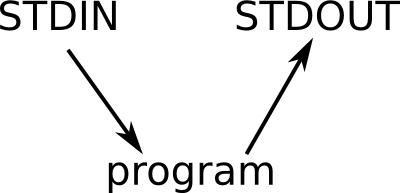
\includegraphics[width=4cm]{asset/g1.png}
\end{figure}
\end{frame}

\begin{frame}[fragile]
\frametitle{Penjelasan Tentang STDIO (lanj.)}
\begin{itemize}
  \item Untuk lebih memahami tentang hal ini, coba buat sebuah berkas bernama input.txt pada \textit{folder} yang sama dengan program jumlah.pas, dan berisi:
  \begin{lstlisting}
    1
    2
  \end{lstlisting}
  \item Kemudian pada \textit{command line}, saat menjalankan program jumlah.pas, ketikkan perintah:
  \begin{lstlisting}
    jumlah < input.txt > output.txt
  \end{lstlisting}
  \item Buka output.txt dan perhatikan apa yang tercetak!
\end{itemize}
\end{frame}

\begin{frame}[fragile]
\frametitle{Penjelasan Tentang STDIO (lanj.)}
\begin{itemize}
  \item Isi dari output.txt adalah:
  \begin{lstlisting}
    masukkan nilai a:
    masukkan nilai b:
    hasil dari penjumlahan a dan b: 3
  \end{lstlisting}
  \item Tulisan "masukkan nilai ..." juga ikut tercetak, karena pada kasus ini, \textbf{STDOUT} merupakan berkas output.txt. Segala yang dicetak lewat saluran \textbf{STDOUT} akan dicetak ke output.txt.
  \item Dengan pemahaman yang sama, seluruh masukan yang diberikan adalah lewat \textbf{STDIN}, yang merupakan input.txt. Sehingga masukannya perlu dimasukkan ke input.txt terlebih dahulu.
\end{itemize}
\end{frame}

\begin{frame}
\frametitle{Masukan dan Keluaran pada OSN/IOI}
\begin{itemize}
  \item Setelah kalian memahami tentang \textbf{STDIN} dan \textbf{STDOUT}, mungkin kalian sudah bisa menebak kenapa pada OSN/IOI tidak boleh mencetak informasi masukan seperti "masukkan nilai ...".
  \item Hal ini dikarenakan tulisan itu akan ikut tercetak sebagai keluaran, yang mana mengakibatkan ada keluaran yang tidak sesuai spesifikasi soal. Hasilnya, program akan dinilai \alert{\textit{wrong answer}}, alias menghasilkan jawaban yang tidak sesuai.
\end{itemize}
\end{frame}

\begin{frame}
\frametitle{Selanjutnya...}
\begin{itemize}
  \item Kini kalian sudah mempelajari tentang variabel, ekspresi, dan masukan/keluaran.
  \item Artinya, sudah waktunya untuk menulis program-program sederhana.
\end{itemize}
\end{frame}

\end{document}
